\documentclass[11pt,a4paper]{article}
\usepackage[a4paper,margin=21mm,headheight=15pt]{geometry}
\usepackage{graphicx,booktabs,longtable,tabularx,amsmath,amssymb,fancyhdr,hyperref,microtype}
\usepackage[font=small,labelfont=bf]{caption}
\usepackage{enumitem}
\hypersetup{colorlinks=true,linkcolor=blue,urlcolor=blue}
\pagestyle{fancy}\fancyhf{}\lhead{LION PCM | paired comparison}\rhead{28 October 2026}\cfoot{\thepage}
\setlength{\parskip}{5pt}\setlength{\parindent}{0pt}
\newcommand{\mes}{\ensuremath{10^{3}\!\times\!\mathrm{MSE}}}
\begin{document}
\begin{center}
{\LARGE\bfseries Full comparison of 4070 and 4090 trainings}\\[7pt]
{\Large 50-image repeat: previous and current checkpoints}\\[7pt]
LION / PCM supervised U-TV reconstruction\\[4pt]
28 October 2026 | RTX 4070 evaluation on tuni
\end{center}
\hrule\vspace{6pt}
\begin{abstract}
A fully paired comparison on 50 test images (10 sampled without replacement per category), under two predeclared PCM noise regimes. The previous frozen checkpoints (4070 epoch 7, 4090 epoch 22) and current validation-selected checkpoints (4070 epoch 17, 4090 epoch 23) are compared on the exact same 100 acquisitions. The original measurement hashes are reproduced exactly. Two hundred current-checkpoint reconstructions were run on the RTX 4070; the previous checkpoint metrics were reused from the complete 27 October test. Reported confidence intervals use 20,000 paired, category-stratified bootstrap resamples. The images were held out from training and validation but were already used in the earlier full test, so this repeat must not be represented as a new untouched test-set confirmation.
\end{abstract}
\tableofcontents\clearpage
\section{Executive summary}

\begin{itemize}[leftmargin=*]
\item \textbf{4070:} balanced MSE decreases by 10.0\% (2.717 to 2.445 in units of $10^{-3}$); PSNR increases by 0.378 dB. MSE paired 95\% CI: [-0.532, -0.075].
\item \textbf{4090:} balanced MSE decreases by 1.8\% (2.594 to 2.549 in units of $10^{-3}$); PSNR and SSIM decline on average. The paired MSE interval [-0.361, +0.189] contains zero.
\item \textbf{Current head-to-head:} 4070 is ahead on all four average metrics. The 4090-minus-4070 MSE interval [-0.022, +0.207] ($\times 10^{-3}$) includes zero; the MSE mean ranking is not resolved convincingly by this 50-image sample.
\item \textbf{Important qualification:} the same 450-image test partition was already evaluated on 27 October. This is a predeclared random subset to track checkpoint progress on matched measurements, not a new external validation of model-selection choices.
\end{itemize}
\section{Protocol and reproducibility}
\textbf{Test split.} The original configuration uses permuted positions 1--900 for training, 901--910 for validation, and 911--1000 for test. Exactly 10 of the 90 test IDs per category were drawn with no replacement, independently within CIGS, Organic, Perovskite, Reference and Silicone. A single fixed random seed namespace was recorded before evaluation, and the same 50 images were used for all checkpoints. There was no selection based on reconstruction results.

\textbf{Forward model.} PCM normalized operator, 256-by-256 reference images, multilevel Hadamard patterns at $J=8$ and coarse level $J=6$, with each image's sampling ratio drawn uniformly from $[0.05,0.50]$. One acquisition per image per noise condition, for a total of 100 acquisitions. Both U-TV models reconstruct the exact same measurement object for each acquisition. All 100 measurement and pattern hashes matched the earlier evaluation.

\textbf{Noise regimes.} \emph{Zero-inclusive} draws raw dark noise on $[0,10^{-5}]$, bias on $[0,4\cdot 10^{-5}]$, bias gradient on $[0,2\cdot10^{-7}]$ and beam on $[0,6\cdot10^{-4}]$, each via shifted log-uniform. The lower bound is zero but the continuous sampler need not yield exactly zero. \emph{Positive} uses log-uniform raw dark noise $[10^{-8},10^{-5}]$ and uniform bias $[2\cdot10^{-5},4\cdot10^{-5}]$, bias gradient $[10^{-7},2\cdot10^{-7}]$, beam $[10^{-4},6\cdot10^{-4}]$. The original physical model-to-current conversion is unchanged.

\textbf{Checkpoints.} All four are 4-block U-Nets with 128 initial filters and 512 unrolled PDHG iterations. The current checkpoint was selected before this subset's evaluation from each run's existing validation procedure; no change was made to ongoing training. The older 4090 job uses stochastic validation acquisitions and different optimizer/noise settings, which complicates causal attribution.

\textbf{Uncertainty.} Each bootstrap draw resamples 10 full image units with replacement within each of the five categories (20,000 draws). Its unit is an image with both noise acquisitions and all checkpoints paired. Reported 95\% intervals are percentile intervals for paired mean differences; they reflect subset sampling variation, not train-seed or synthetic-generator uncertainty. This is not a new, unseen-test confirmation because the full test partition was examined previously.

\begin{table}[ht]\centering\caption{Frozen checkpoints; old snapshots from 27 October and new snapshots frozen before this repeat.}\small
\begin{tabular}{lrrl}\toprule Checkpoint & Epoch & Optimizer steps & Selection \\ \midrule
4070 old & 7 & 31,500 & Training validation \\
4070 new & 17 & 76,500 & Training validation \\
4090 old & 22 & 99,000 & Training validation \\
4090 new & 23 & 103,500 & Training validation \\
\bottomrule\end{tabular}\end{table}
\textbf{Source commit:} \texttt{9188b0735843c96526537b6b9bfd834fd089f7cd}; the full checkpoint hashes, exact IDs, copied noise settings and acquisition seeds are stored in \texttt{protocol\_manifest\_50.json}.
\section{Overall reconstruction metrics}
\begin{table}[ht]\centering\caption{Mean of the 100 acquisitions, evenly balancing the two noise regimes. MSE columns are scaled by $10^{3}$.}\small
\begin{tabular}{lrrrr}\toprule Checkpoint & \mes & PSNR (dB) & SSIM & HaarPSI \\ \midrule
4070 epoch 7 & 2.717 & 29.597 & 0.7524 & 0.6615 \\
4070 epoch 17 & 2.445 & 29.975 & 0.7732 & 0.6803 \\
4090 epoch 22 & 2.594 & 29.497 & 0.7550 & 0.6446 \\
4090 epoch 23 & 2.549 & 29.131 & 0.7424 & 0.6454 \\
\bottomrule\end{tabular}\end{table}
\textbf{Reading the metrics.} The 4070 checkpoint improves simultaneously in MSE, PSNR, SSIM and HaarPSI, while the 4090 changes in different directions. An improvement in mean MSE can coexist with a loss of mean per-image PSNR because of the nonlinearity of the logarithm, especially if a few high-error acquisitions dominate the mean MSE.
\begin{figure}[p]\centering
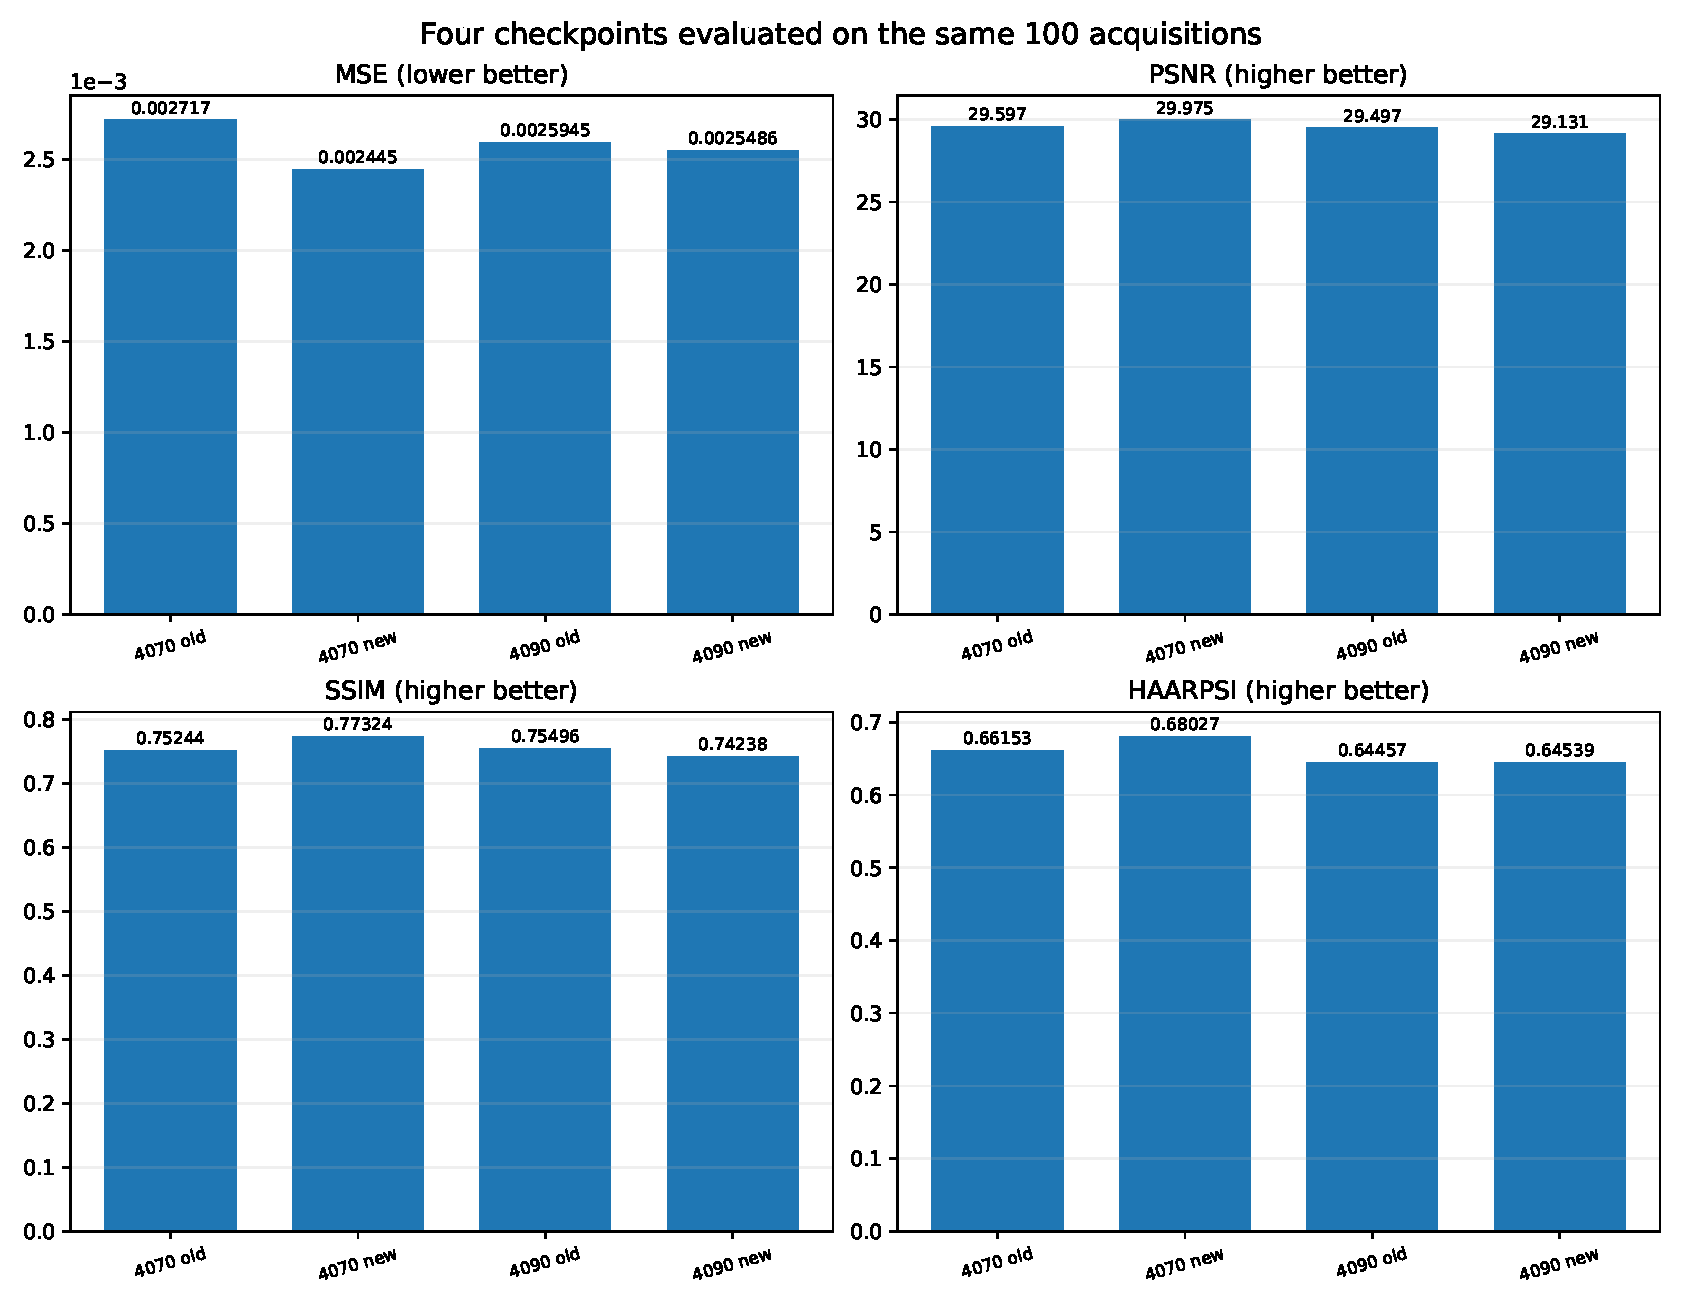
\includegraphics[width=.92\linewidth]{figures/four_checkpoint_means.pdf}
\caption{Four checkpoint means.}
\end{figure}\clearpage
\section{Noise-specific reconstruction results}
\begin{table}[ht]\centering\caption{Mean metrics by acquisition noise regime (50 acquisitions per regime). MSE uses $10^{-3}$ units.}\small
\begin{tabular}{llrrrr}\toprule Regime & Checkpoint & \mes & PSNR & SSIM & HaarPSI \\ \midrule
Zero-inclusive & 4070 old & 2.685 & 29.853 & 0.7540 & 0.6667 \\
Zero-inclusive & 4070 new & 2.374 & 30.288 & 0.7763 & 0.6876 \\
Zero-inclusive & 4090 old & 2.491 & 29.809 & 0.7585 & 0.6513 \\
Zero-inclusive & 4090 new & 2.461 & 29.364 & 0.7453 & 0.6522 \\
\midrule
Positive & 4070 old & 2.749 & 29.342 & 0.7509 & 0.6563 \\
Positive & 4070 new & 2.516 & 29.662 & 0.7702 & 0.6730 \\
Positive & 4090 old & 2.698 & 29.185 & 0.7514 & 0.6378 \\
Positive & 4090 new & 2.636 & 28.899 & 0.7395 & 0.6386 \\

\bottomrule\end{tabular}\end{table}
\textbf{Robustness across noise distributions.} The 4070 gains in all four metrics under both regimes. The latest 4090 gains modestly in mean MSE for both regimes, but mean PSNR and SSIM decline in both. Thus the direction of these changes is not caused solely by averaging the two noise regimes.
\section{Paired changes and uncertainty}
For a difference, \emph{positive} is favorable to the 4090 in the current head-to-head, except for MSE where \emph{negative} is favorable. A negative ``new minus old'' MSE denotes learning progress. Confidence intervals below are calculated on paired image-level units while preserving both acquisitions per image. All figures use 20,000 category-stratified bootstrap samples.
\begin{table}[ht]\centering\small
\caption{Paired MSE differences and 95\% confidence intervals (balanced regimes). Scaled by $10^{3}$.}
\begin{tabular}{lrr}\toprule Comparison & Difference & 95\% CI \\ \midrule
4070: new - old & -0.272 & [-0.532, -0.075] \\
4090: new - old & -0.046 & [-0.361, +0.189] \\
Old: 4090 - 4070 & -0.123 & [-0.240, -0.024] \\
New: 4090 - 4070 & +0.104 & [-0.022, +0.207] \\
Shift in model gap & +0.226 & [+0.093, +0.357] \\
\bottomrule\end{tabular}\end{table}
\begin{table}[ht]\centering\small
\caption{Paired PSNR differences and 95\% confidence intervals (balanced regimes). }
\begin{tabular}{lrr}\toprule Comparison & Difference & 95\% CI \\ \midrule
4070: new - old & +0.378 & [+0.288, +0.468] \\
4090: new - old & -0.366 & [-0.519, -0.216] \\
Old: 4090 - 4070 & -0.100 & [-0.236, +0.038] \\
New: 4090 - 4070 & -0.844 & [-1.000, -0.685] \\
Shift in model gap & -0.744 & [-0.947, -0.542] \\
\bottomrule\end{tabular}\end{table}
\clearpage
\begin{table}[ht]\centering\small
\caption{Paired SSIM differences and 95\% confidence intervals (balanced regimes). }
\begin{tabular}{lrr}\toprule Comparison & Difference & 95\% CI \\ \midrule
4070: new - old & +0.0208 & [+0.0170, +0.0247] \\
4090: new - old & -0.0126 & [-0.0161, -0.0094] \\
Old: 4090 - 4070 & +0.0025 & [-0.0010, +0.0064] \\
New: 4090 - 4070 & -0.0309 & [-0.0367, -0.0253] \\
Shift in model gap & -0.0334 & [-0.0397, -0.0276] \\
\bottomrule\end{tabular}\end{table}
\begin{table}[ht]\centering\small
\caption{Paired HAARPSI differences and 95\% confidence intervals (balanced regimes). }
\begin{tabular}{lrr}\toprule Comparison & Difference & 95\% CI \\ \midrule
4070: new - old & +0.0187 & [+0.0146, +0.0231] \\
4090: new - old & +0.0008 & [-0.0045, +0.0062] \\
Old: 4090 - 4070 & -0.0170 & [-0.0214, -0.0127] \\
New: 4090 - 4070 & -0.0349 & [-0.0422, -0.0279] \\
Shift in model gap & -0.0179 & [-0.0259, -0.0103] \\
\bottomrule\end{tabular}\end{table}
\textbf{Reading the paired results.} The 4070 gains are reasonably consistent across acquisitions in PSNR, SSIM and HaarPSI. The 4090's MSE change interval overlaps zero, while its paired PSNR and SSIM changes favor the older checkpoint. The difference-in-differences indicates that the relative gap between 4070 and 4090 shifted toward the 4070, although the current mean MSE head-to-head comparison itself has an interval including zero. The two statements are compatible: change in relative performance is measured more precisely than the remaining gap.
\begin{figure}[p]\centering
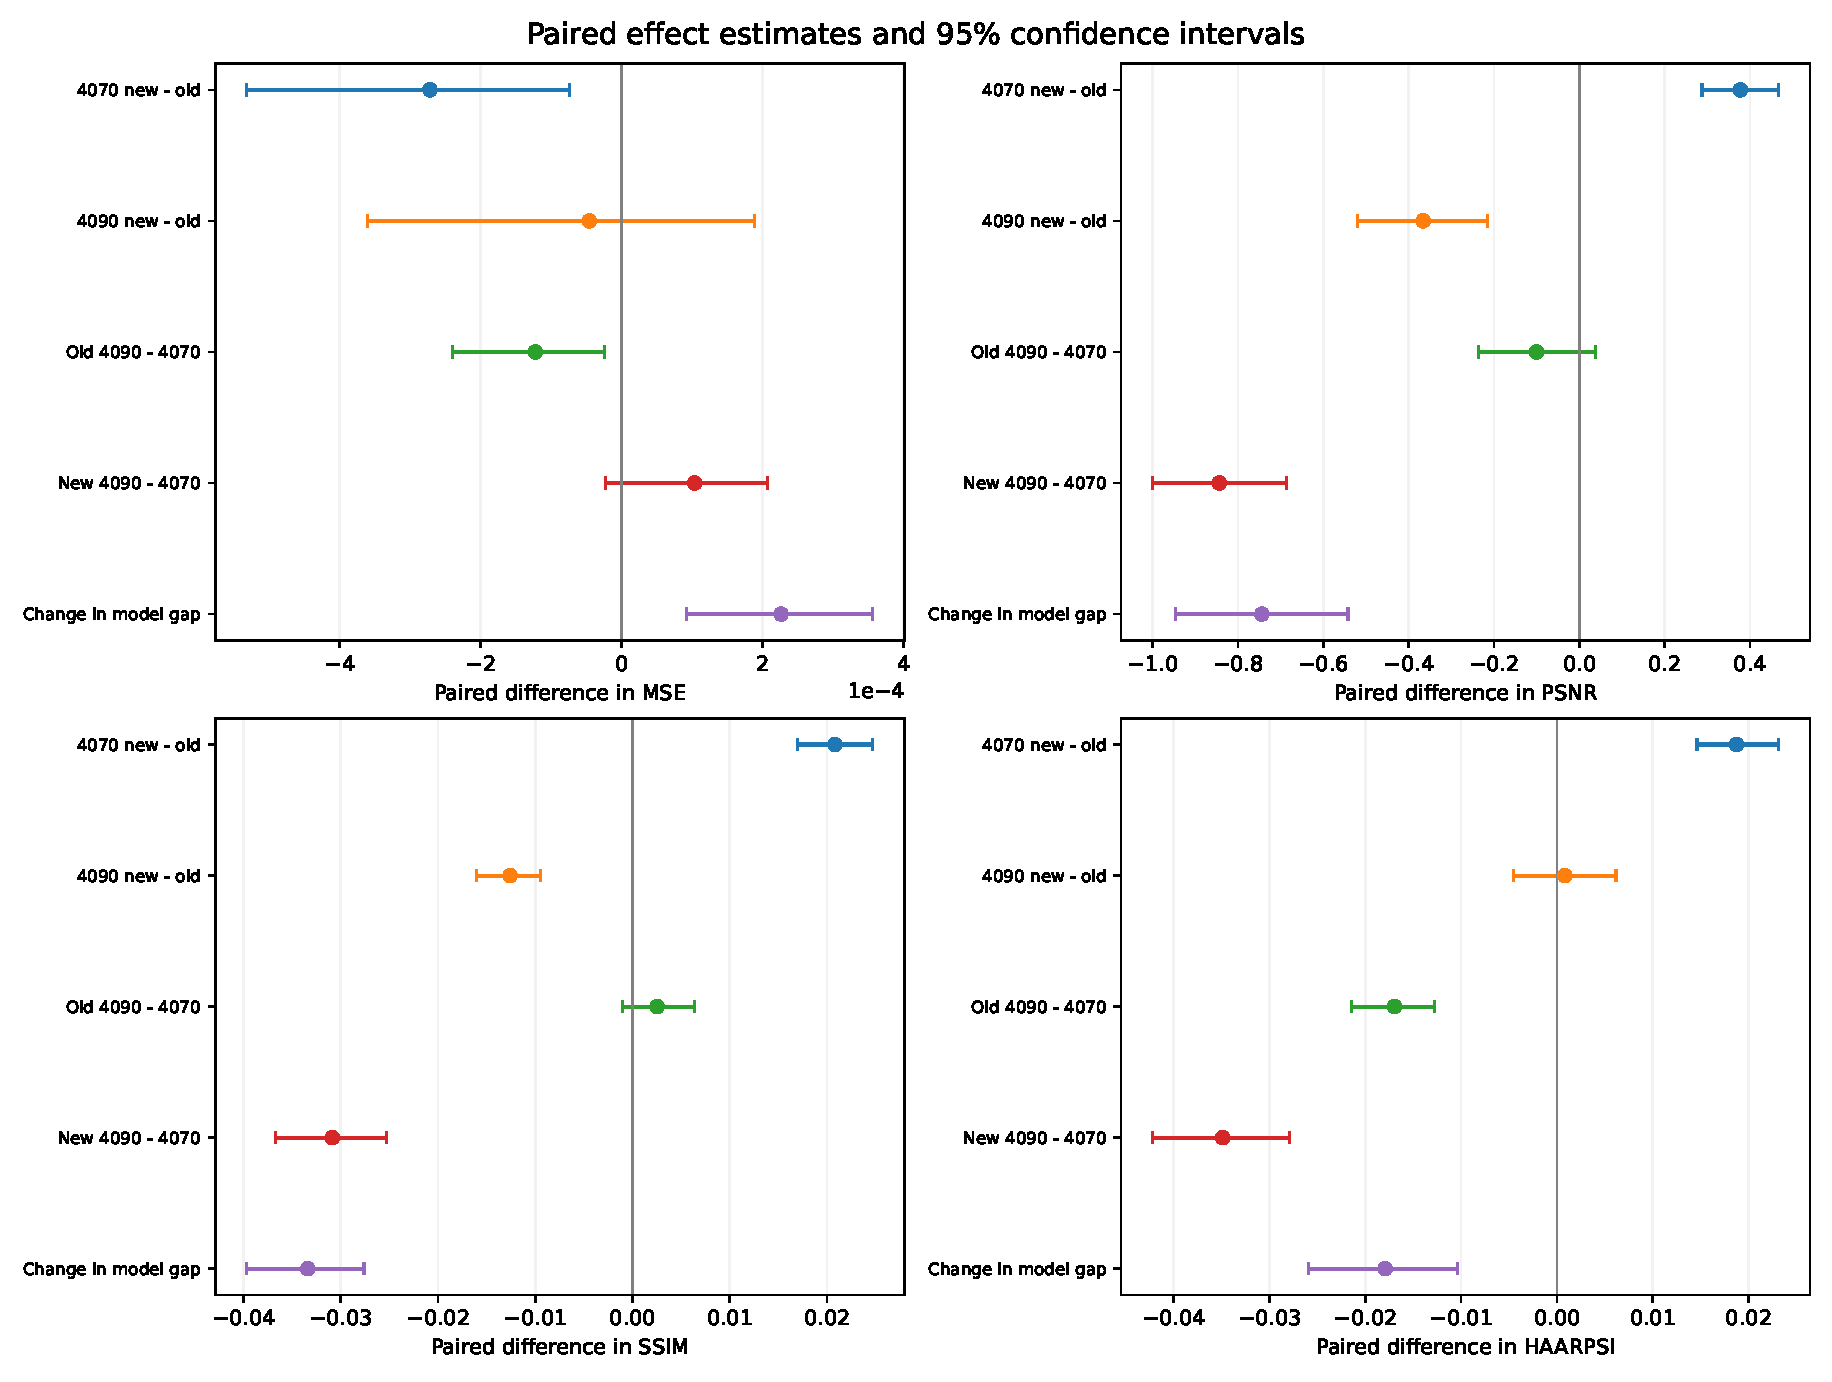
\includegraphics[width=.91\linewidth]{figures/paired_effect_confidence_intervals.pdf}
\caption{Paired effect confidence intervals.}
\end{figure}\clearpage
\section{Category and sampling heterogeneity}
\begin{table}[ht]\centering\caption{Current-checkpoint mean errors by category and noise regime. Negative gap is favorable to 4090. MSE numbers are $\times10^{-3}$.}\footnotesize
\begin{tabular}{llrrr}\toprule Category & Noise & 4070 MSE & 4090 MSE & Gap (4090 - 4070) \\ \midrule
CIGS & Zero & 1.376 & 1.570 & +0.194 \\
CIGS & Positive & 0.841 & 1.034 & +0.193 \\
\addlinespace
Organic & Zero & 0.895 & 0.911 & +0.016 \\
Organic & Positive & 0.313 & 0.369 & +0.056 \\
\addlinespace
Perovskite & Zero & 1.550 & 1.498 & -0.051 \\
Perovskite & Positive & 3.944 & 3.562 & -0.382 \\
\addlinespace
Reference & Zero & 5.146 & 4.924 & -0.223 \\
Reference & Positive & 3.108 & 3.286 & +0.178 \\
\addlinespace
Silicone & Zero & 2.901 & 3.402 & +0.501 \\
Silicone & Positive & 4.376 & 4.930 & +0.554 \\
\bottomrule\end{tabular}\end{table}
\textbf{Heterogeneity.} A positive aggregated MSE gap does not imply that one checkpoint wins on every type of image. Some categories and sampling ratios favor the 4090. The paired distribution figure reveals whether the average is sensitive to a small number of large errors; do not interpret the 50-image mean as a category-independent effect.
\begin{figure}[p]\centering
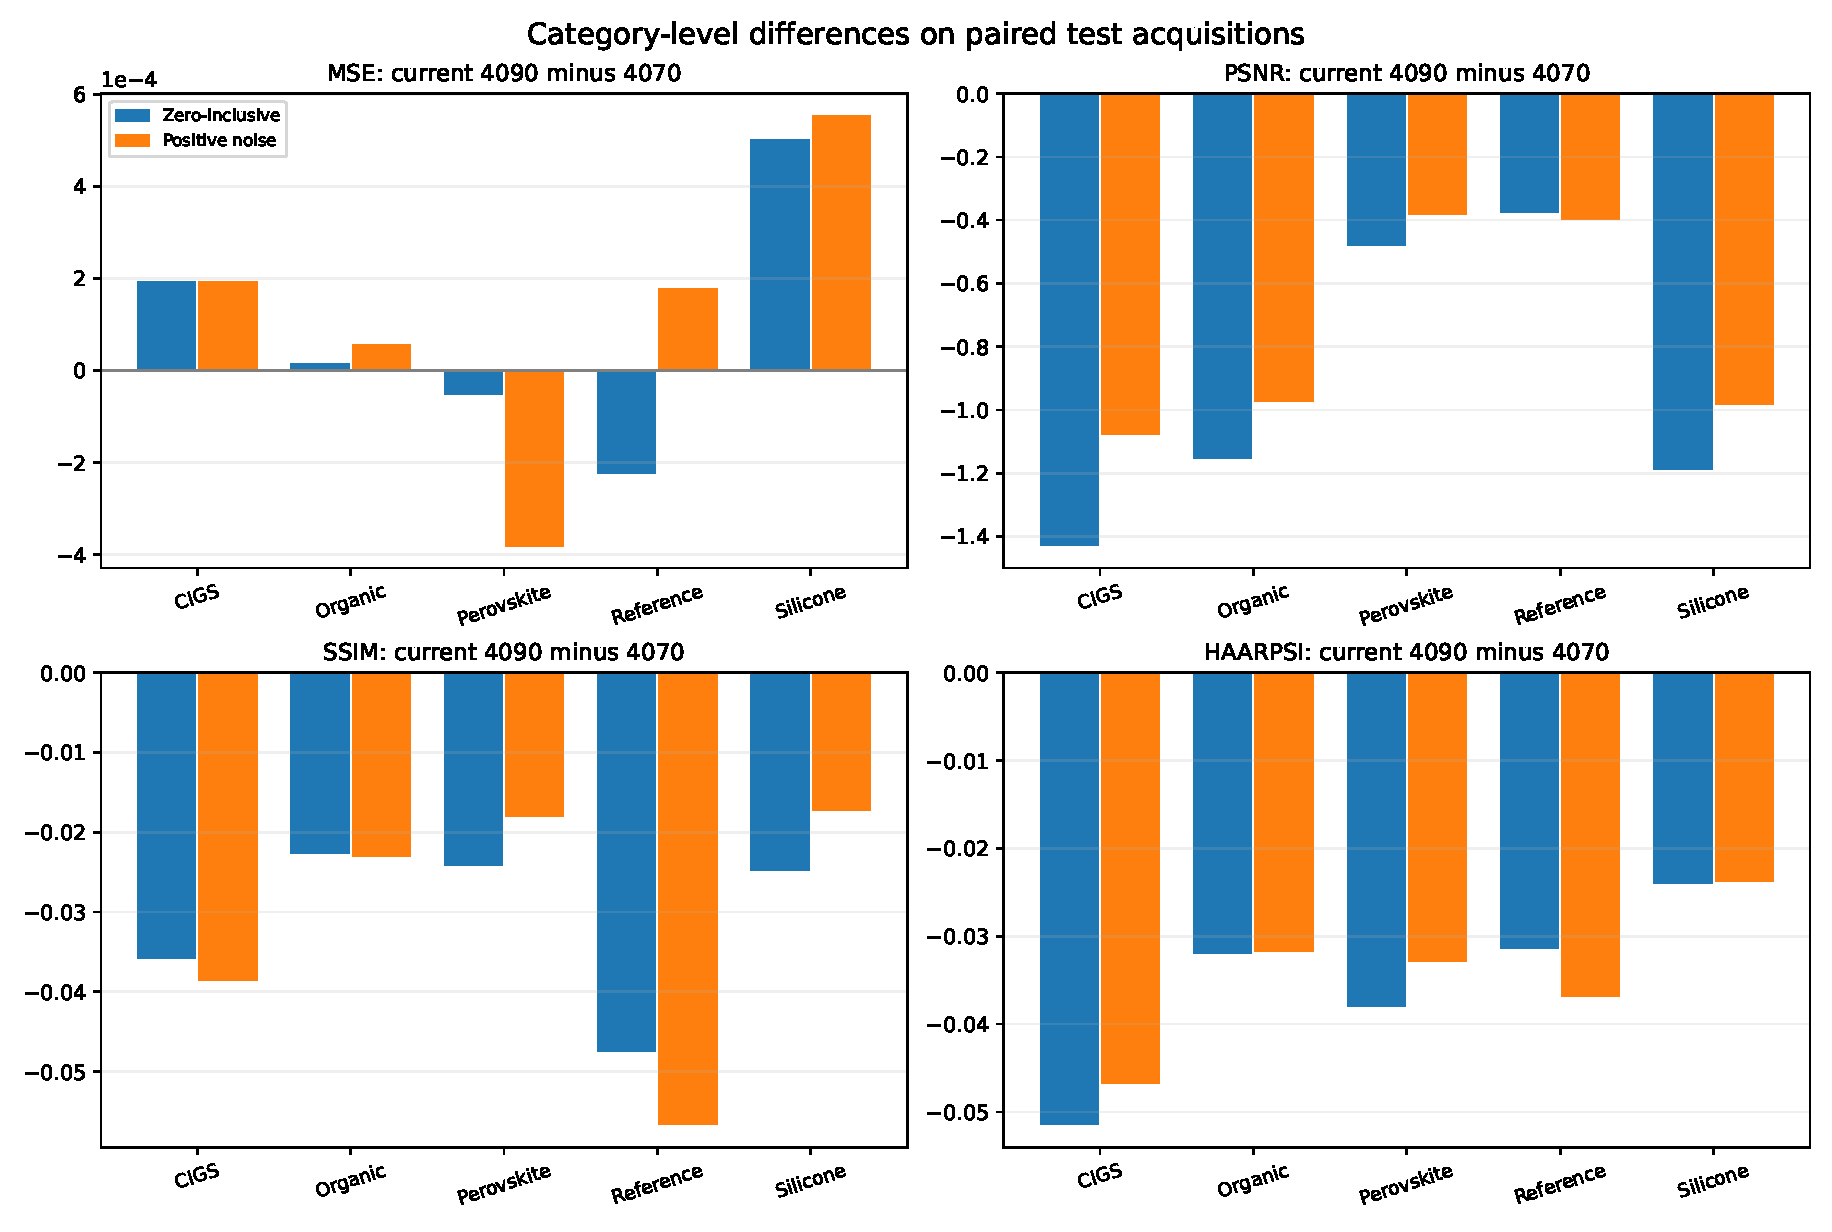
\includegraphics[width=.91\linewidth]{figures/category_by_noise.pdf}
\caption{Category by noise.}
\end{figure}\clearpage
\begin{table}[ht]\centering\caption{MSE changes stratified by sampling ratio (scaled by $10^3$). Small bin counts mean exploratory results.}\small
\begin{tabular}{lrrrr}\toprule Sampling ratio & Images & New gap & 4070 new - old & 4090 new - old \\ \midrule
0.05-0.15 & 13 & -0.176 & -0.886 & -0.653 \\
0.15-0.25 & 10 & +0.221 & -0.142 & +0.164 \\
0.25-0.35 & 13 & +0.203 & -0.042 & +0.179 \\
0.35-0.50 & 14 & +0.188 & -0.009 & +0.159 \\
\bottomrule\end{tabular}\end{table}
\begin{figure}[p]\centering
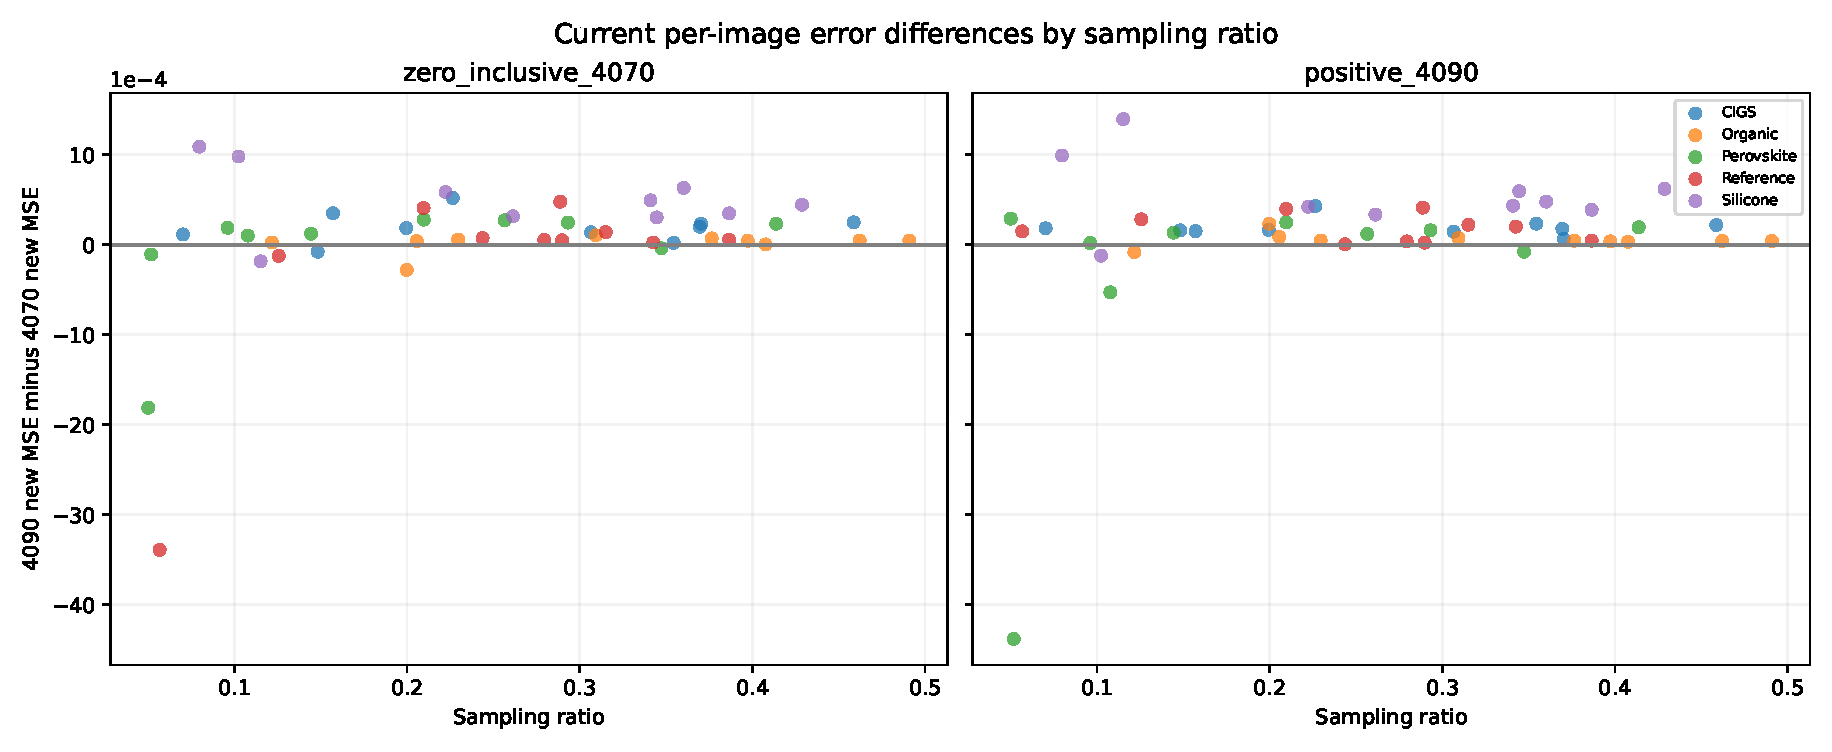
\includegraphics[width=.90\linewidth]{figures/mse_difference_vs_sampling.pdf}
\caption{Mse difference vs sampling.}
\end{figure}\clearpage
\section{How often each model wins}
\begin{table}[ht]\centering\caption{Acquisition-level wins for the current 4090 versus current 4070 (50 acquisitions per regime).}\small
\begin{tabular}{llrrr}\toprule Noise regime & Metric & 4070 wins & 4090 wins & Ties \\ \midrule
Zero-inclusive & MSE & 42 & 8 & 0 \\
Zero-inclusive & PSNR & 42 & 8 & 0 \\
Zero-inclusive & SSIM & 45 & 5 & 0 \\
Zero-inclusive & HAARPSI & 43 & 7 & 0 \\
\midrule
Positive & MSE & 45 & 5 & 0 \\
Positive & PSNR & 45 & 5 & 0 \\
Positive & SSIM & 46 & 4 & 0 \\
Positive & HAARPSI & 44 & 6 & 0 \\

\bottomrule\end{tabular}\end{table}
The win counts and mean differences answer different questions. A model may win on most cases while losing the \emph{mean MSE} because its losses on a few difficult images are much larger. PSNR, SSIM and HaarPSI are therefore essential alongside mean MSE. Each acquisition yields one deterministic paired comparison; these counts are not independent replications of training.
\begin{figure}[p]\centering
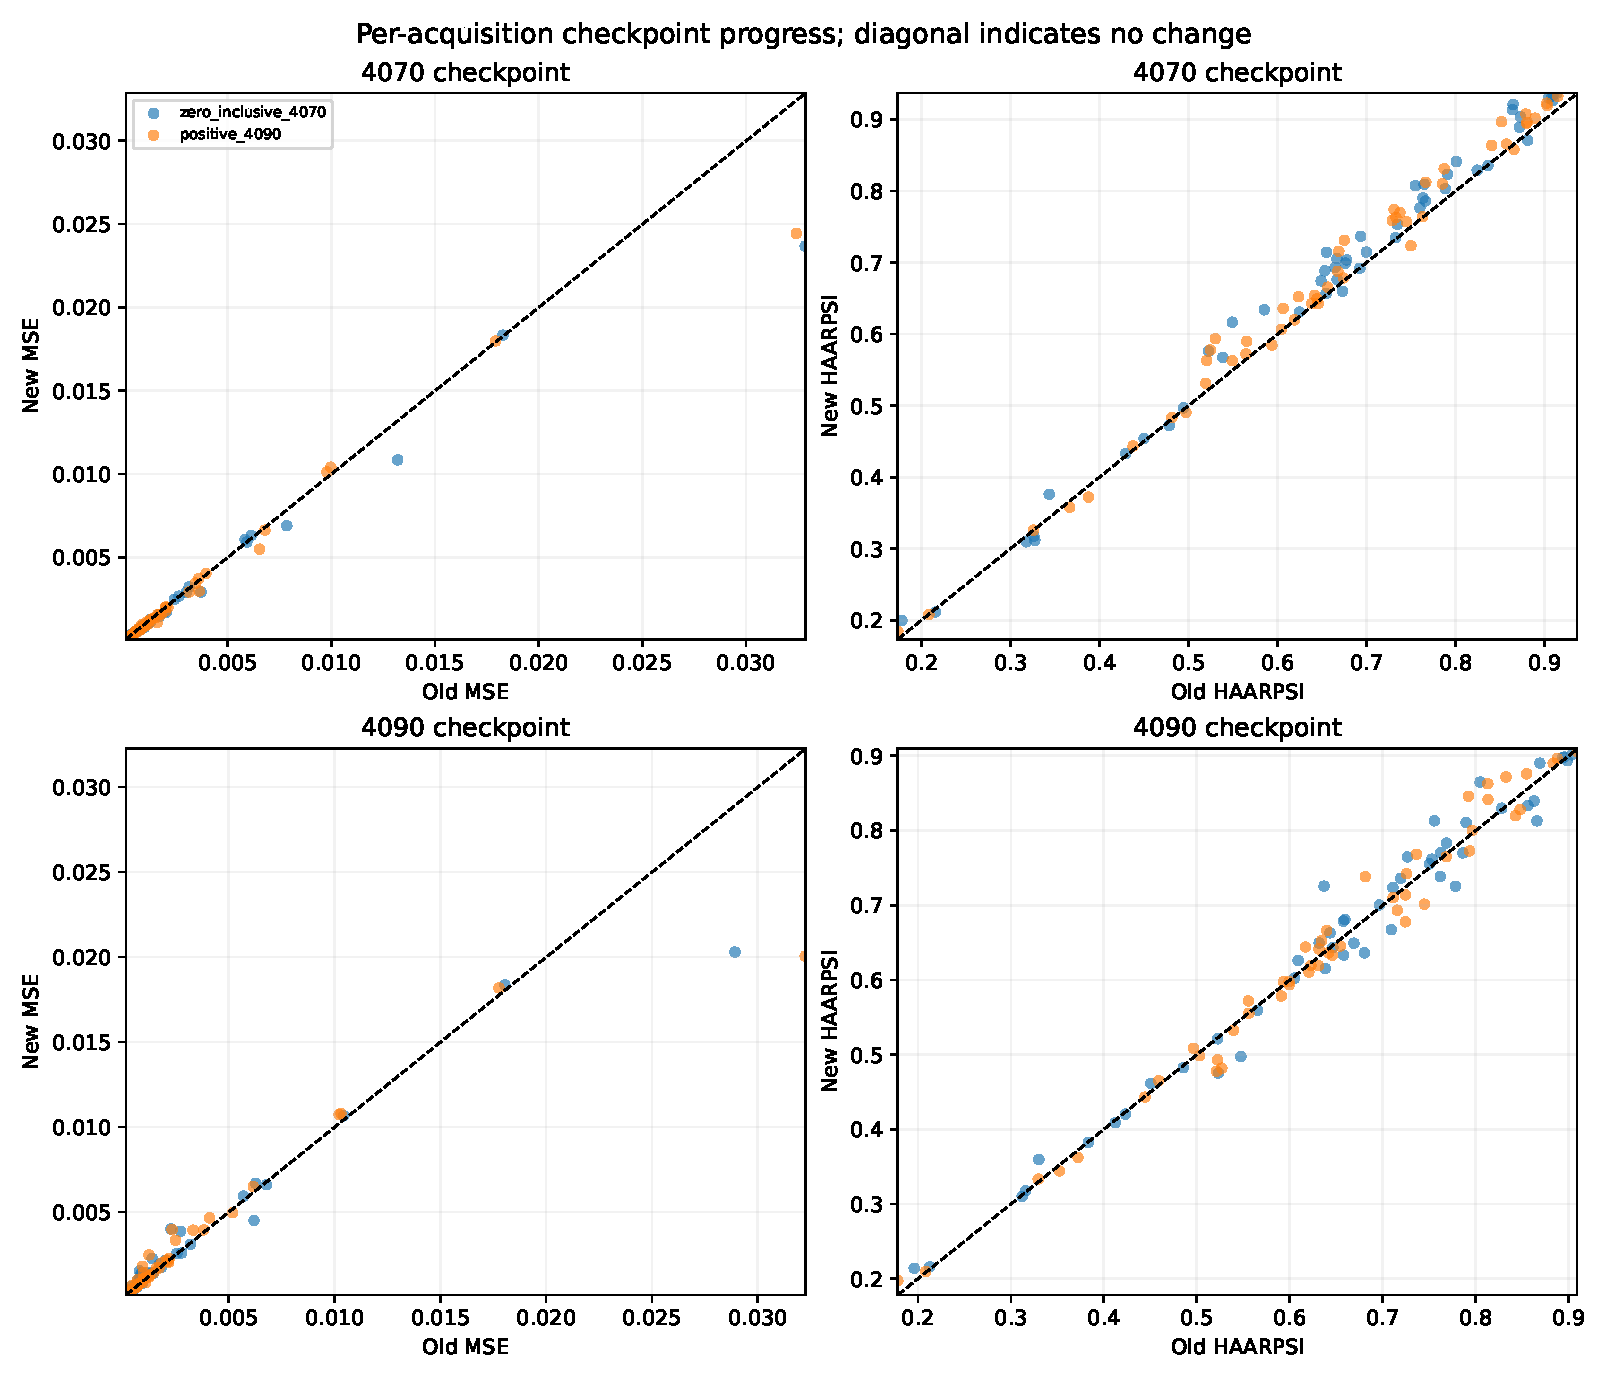
\includegraphics[width=.90\linewidth]{figures/paired_old_new_scatter.pdf}
\caption{Paired old new scatter.}
\end{figure}\clearpage
\section{Qualitative reconstruction assessment}
For each category, the illustrative image is the \emph{first of the ten preselected random IDs}, not an outcome-dependent best or worst case. Each panel displays the same normalized intensity scale, $[0,1.2]$, using the afmhot colormap. The zero-filled image is included as a reconstruction reference. The newly trained 4070 and 4090 checkpoints both receive the identical acquisition. Individual image panels are embedded in a PDF figure without first flattening them into a giant low-resolution bitmap. Numerical PSNR is displayed adjacent to reconstructions. The qualitative comparisons serve as examples; the tables reflect all 50 images, not merely these examples.
\begin{figure}[p]\centering
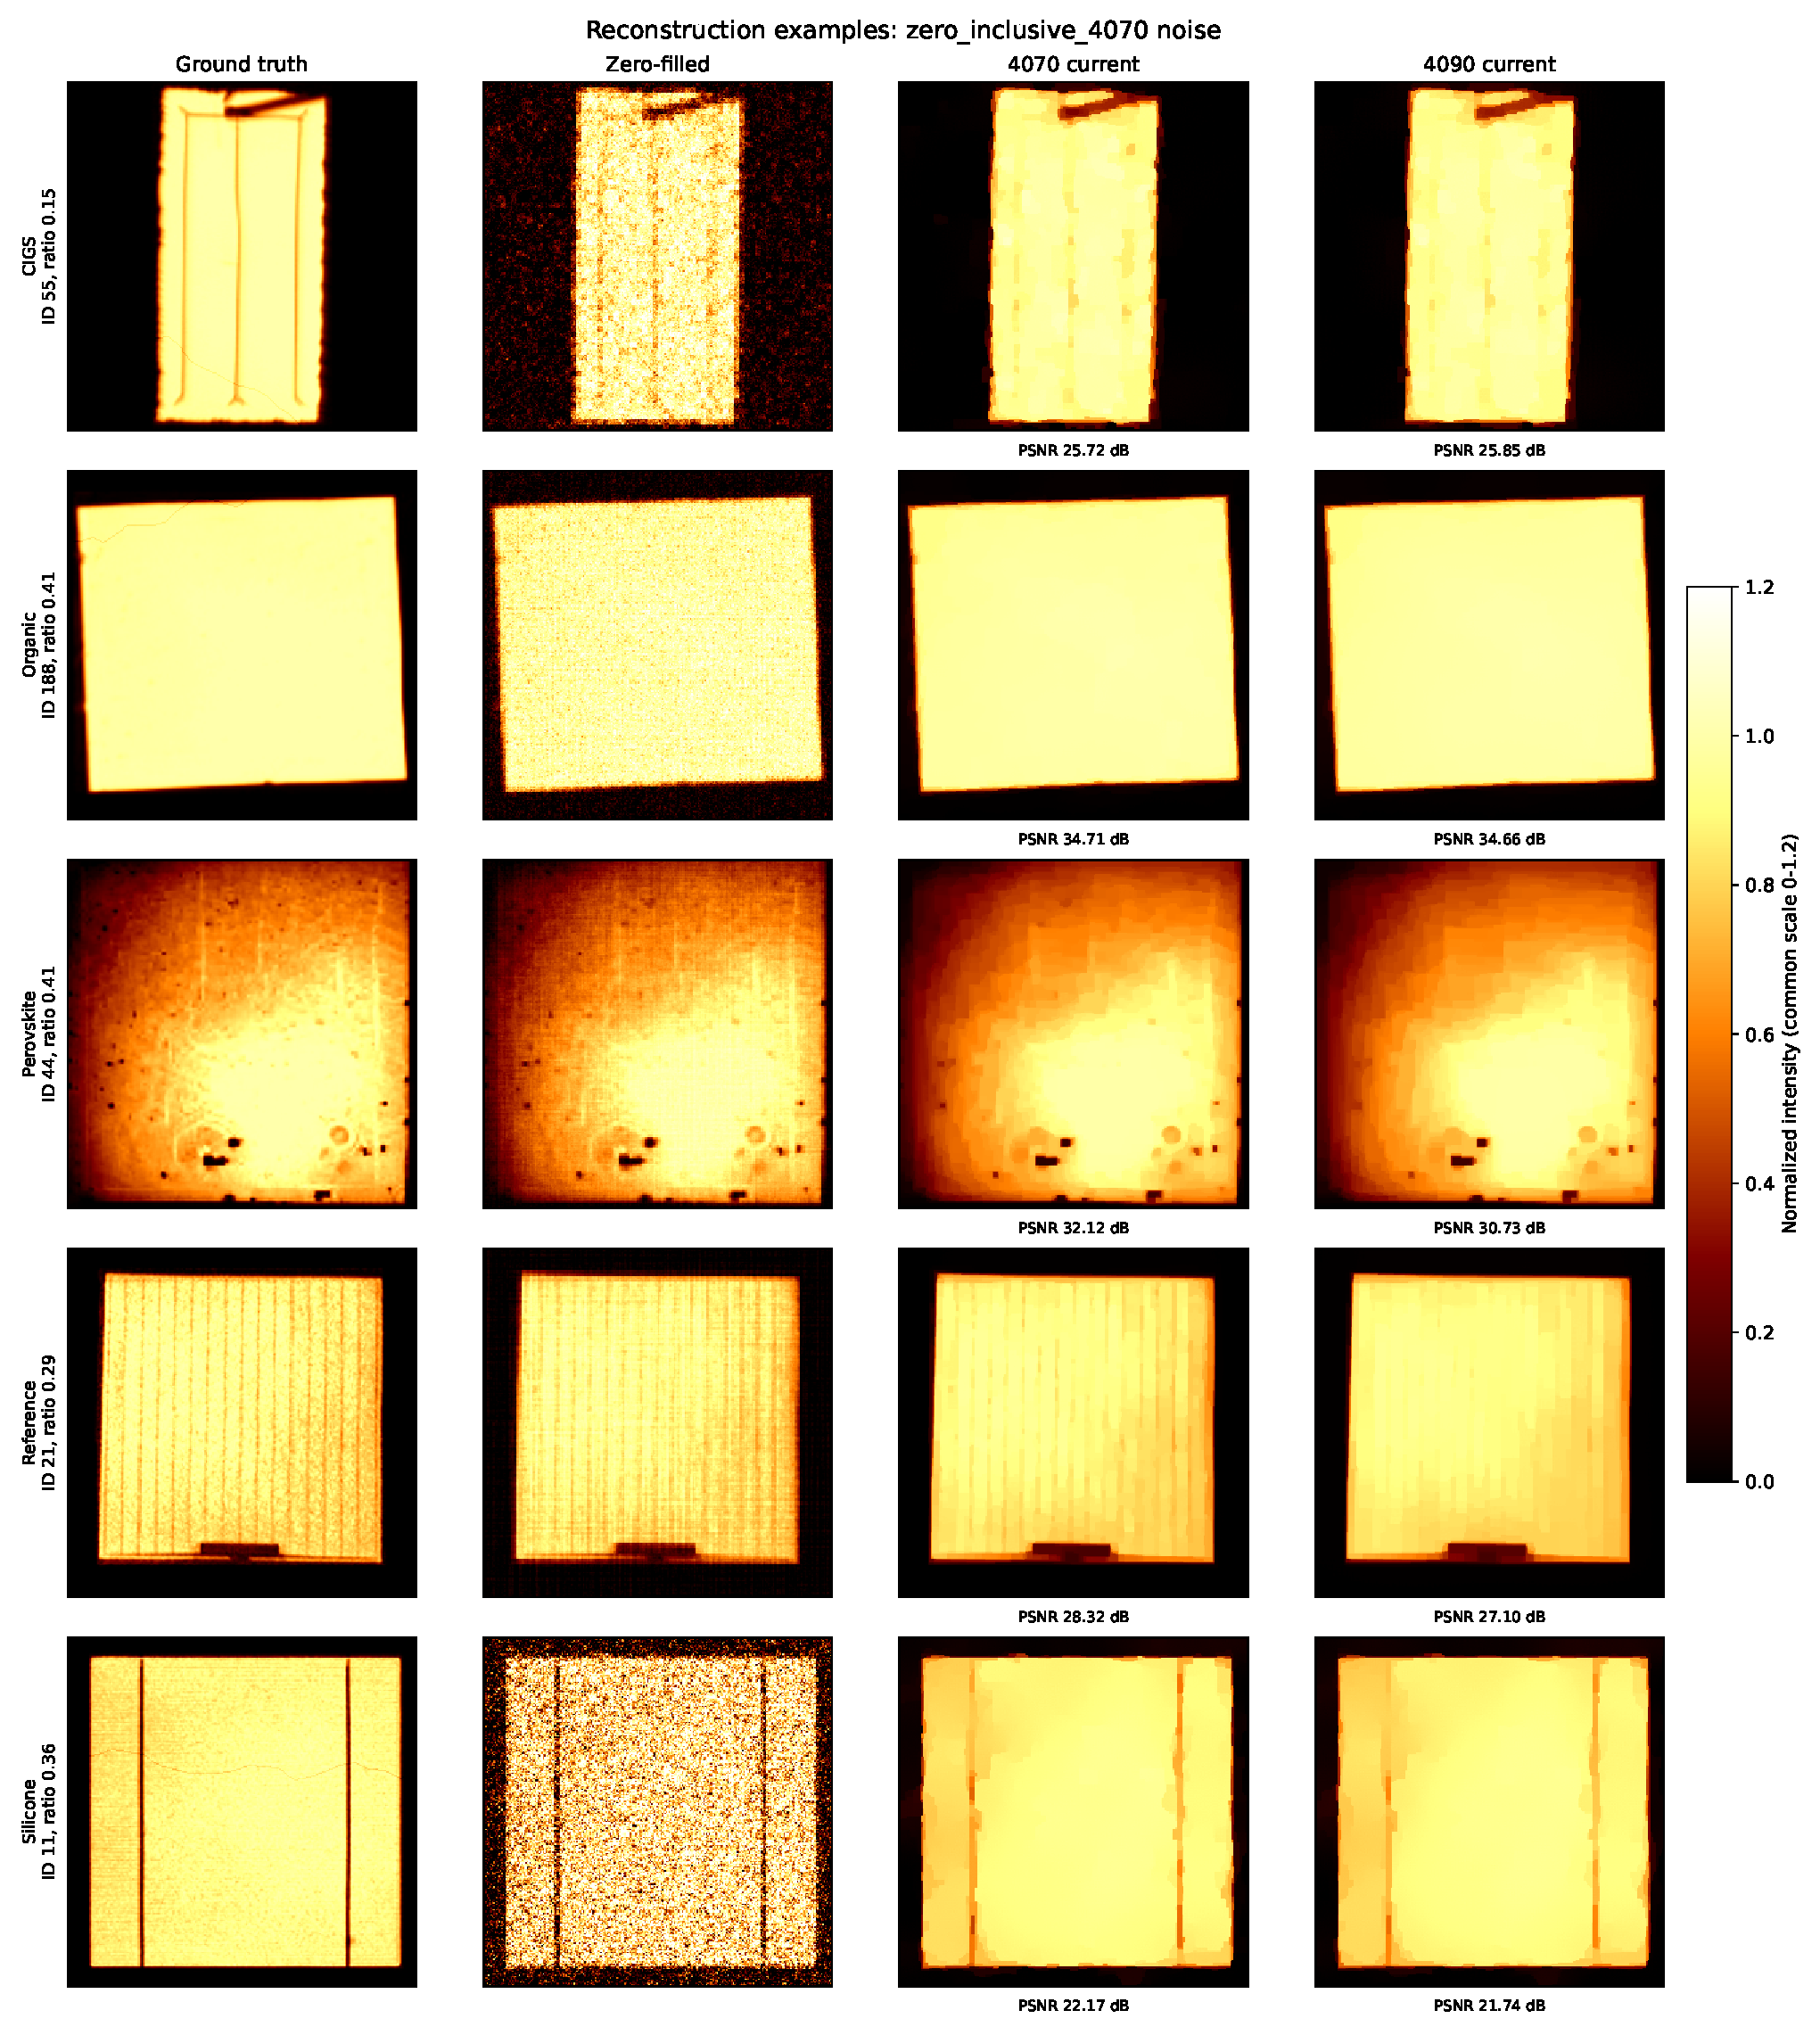
\includegraphics[width=.80\linewidth]{figures/reconstructions_zero_inclusive_4070.pdf}
\caption{Reconstructions zero inclusive 4070.}
\end{figure}\clearpage
\begin{figure}[p]\centering
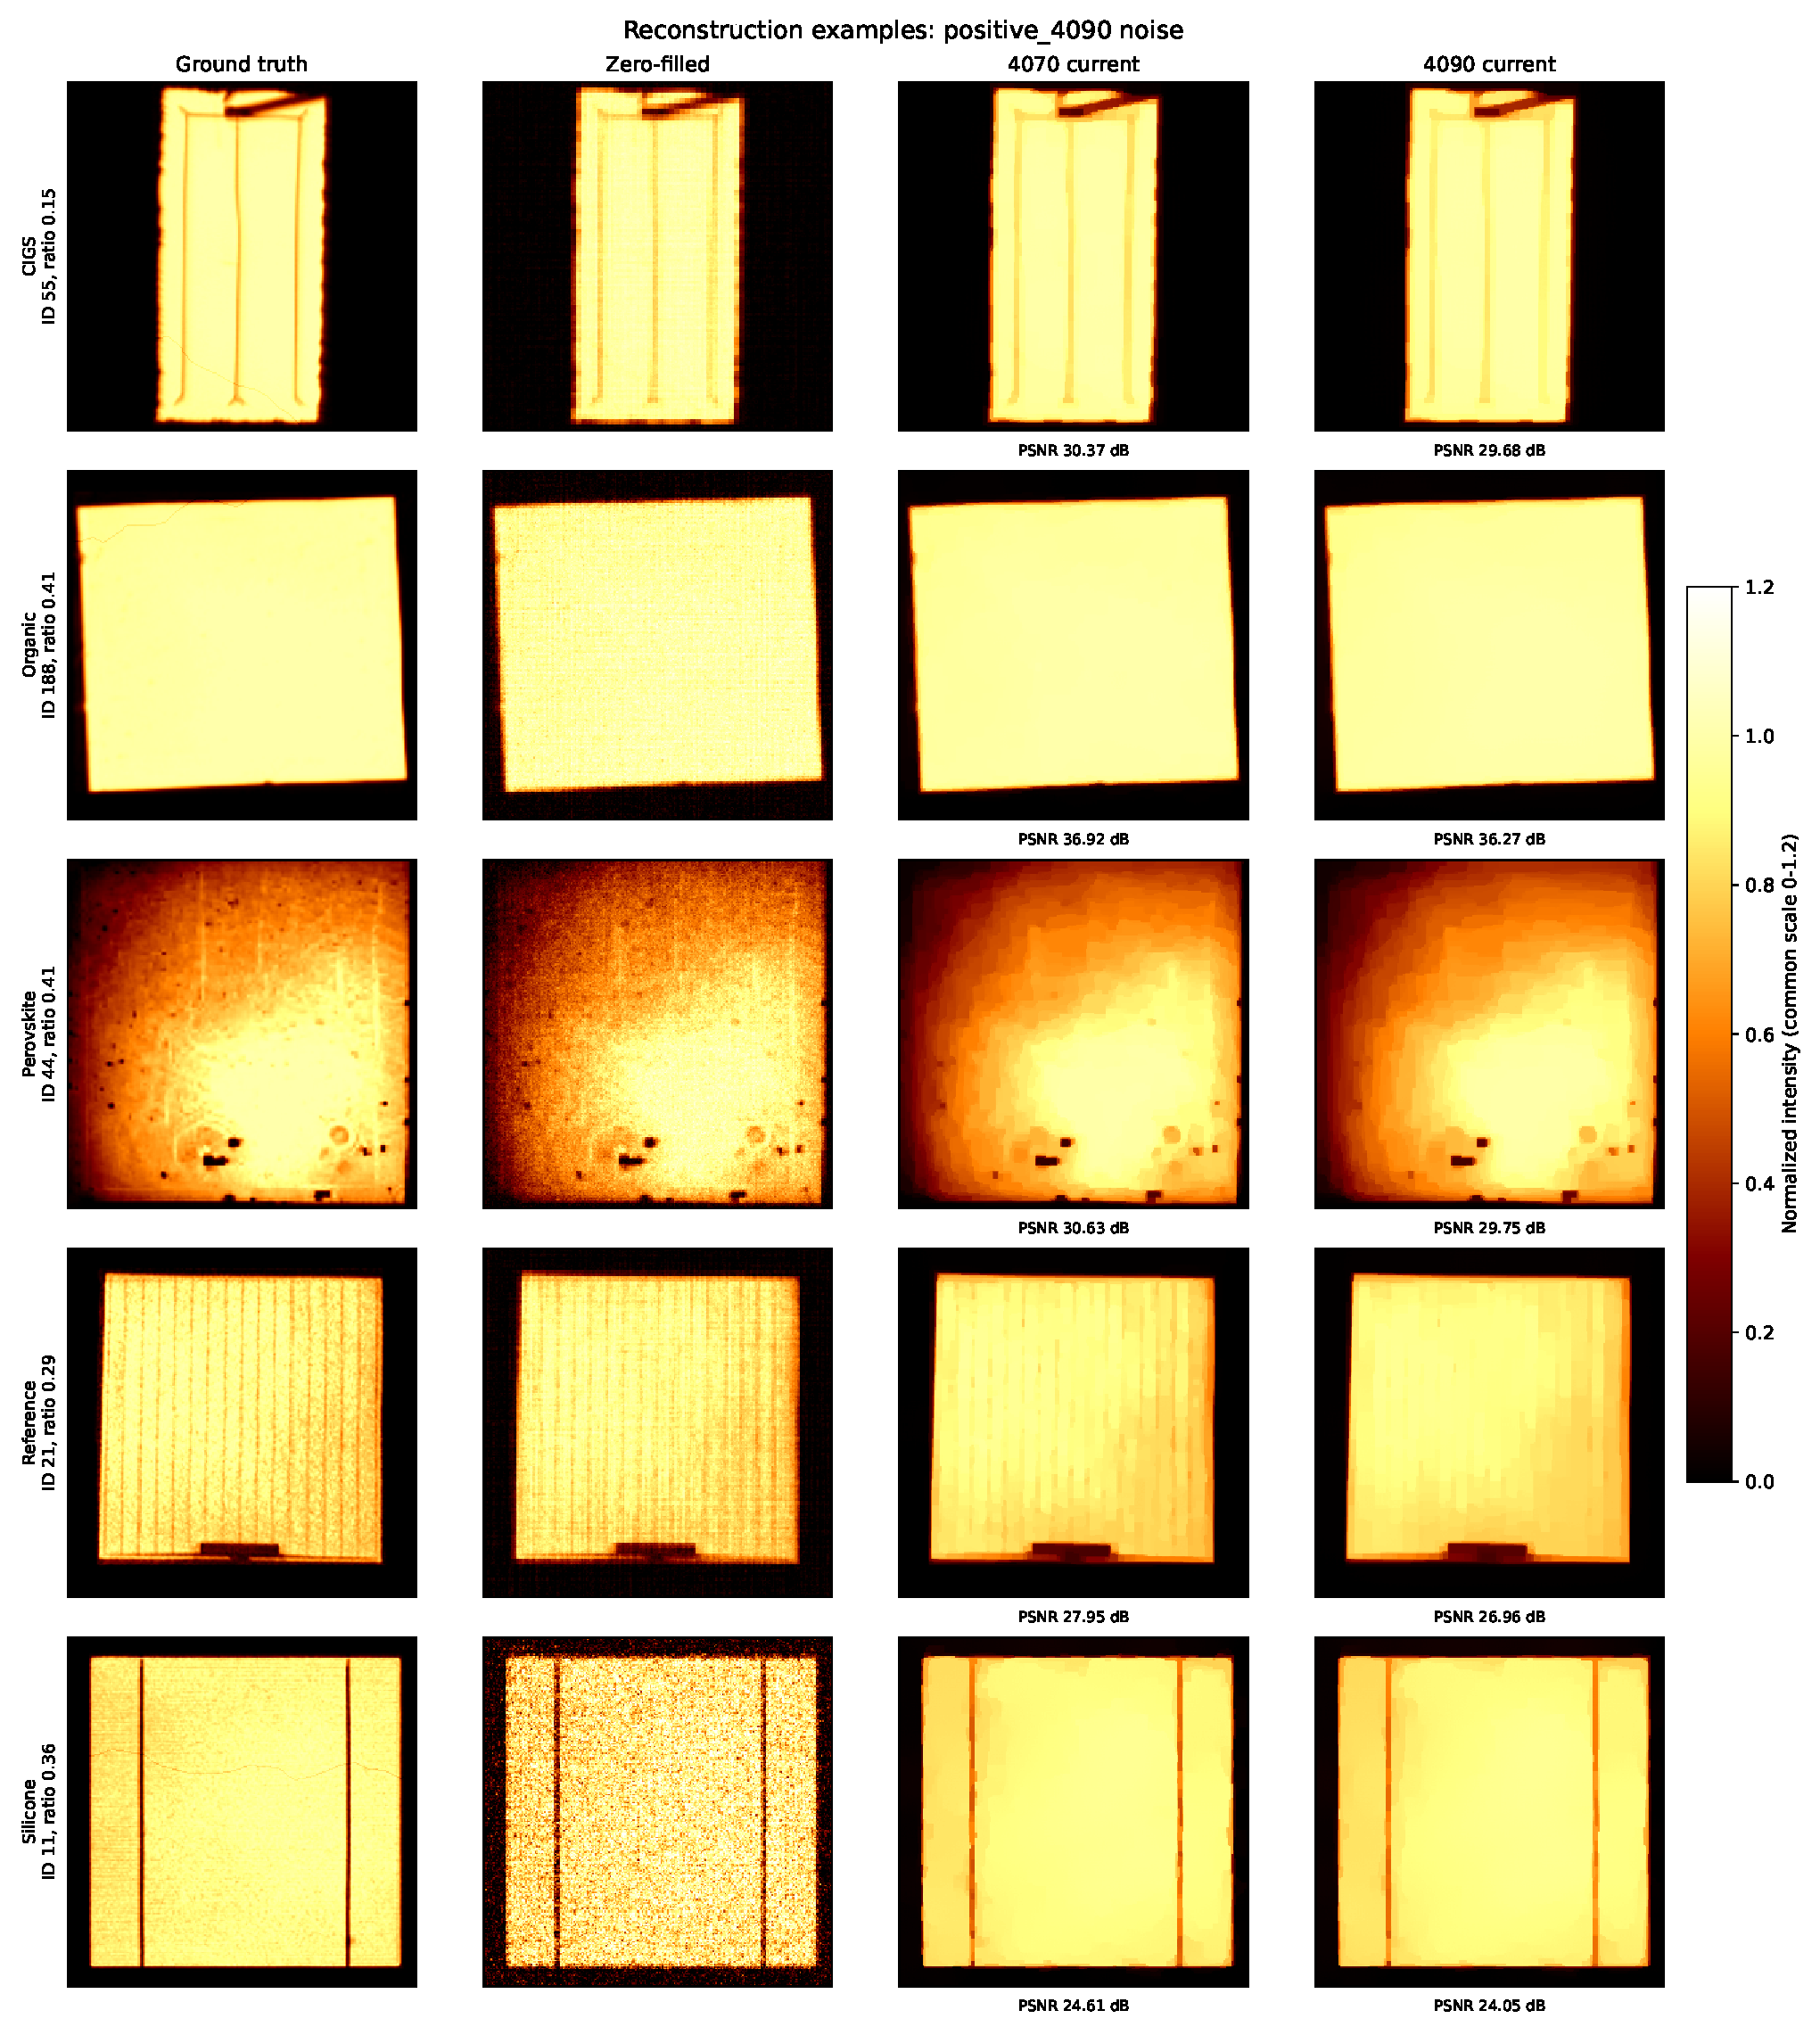
\includegraphics[width=.80\linewidth]{figures/reconstructions_positive_4090.pdf}
\caption{Reconstructions positive 4090.}
\end{figure}\clearpage
\subsection{Absolute error on common scales}
The following figures use absolute errors with the same linear color scale $[0,0.5]$ for \emph{all} displayed categories, noise regimes and models. This prevents a model with larger errors from appearing artificially similar through independent auto-rescaling. The display can clip larger errors, so numeric MSE and the detailed per-image CSV remain the quantitative reference.
\begin{figure}[p]\centering
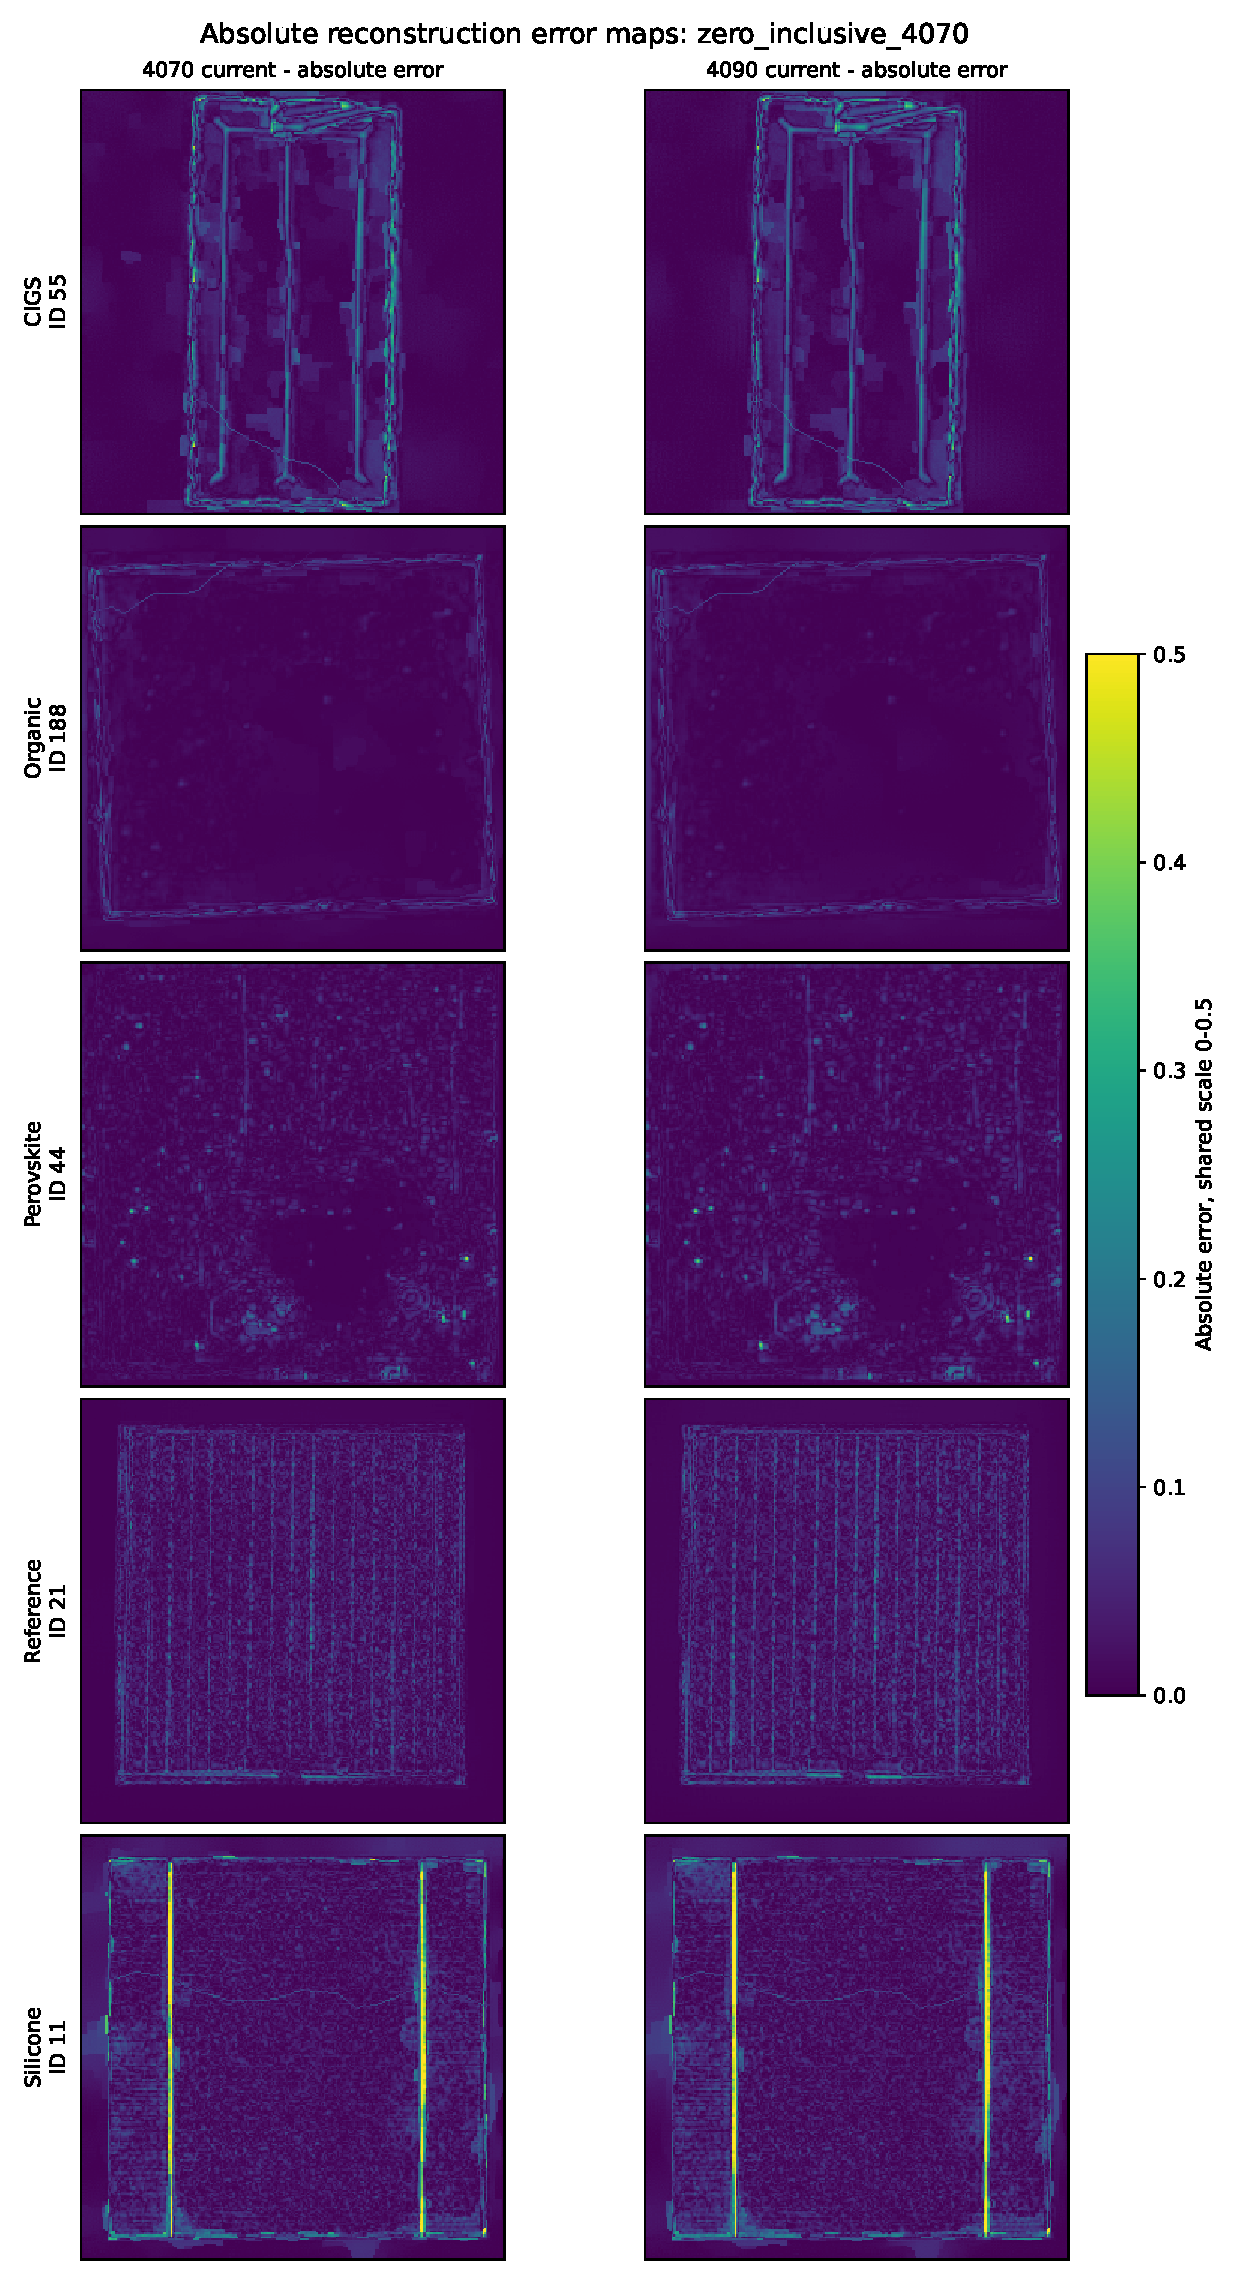
\includegraphics[width=.56\linewidth]{figures/absolute_error_zero_inclusive_4070.pdf}
\caption{Absolute error zero inclusive 4070.}
\end{figure}\clearpage
\begin{figure}[p]\centering
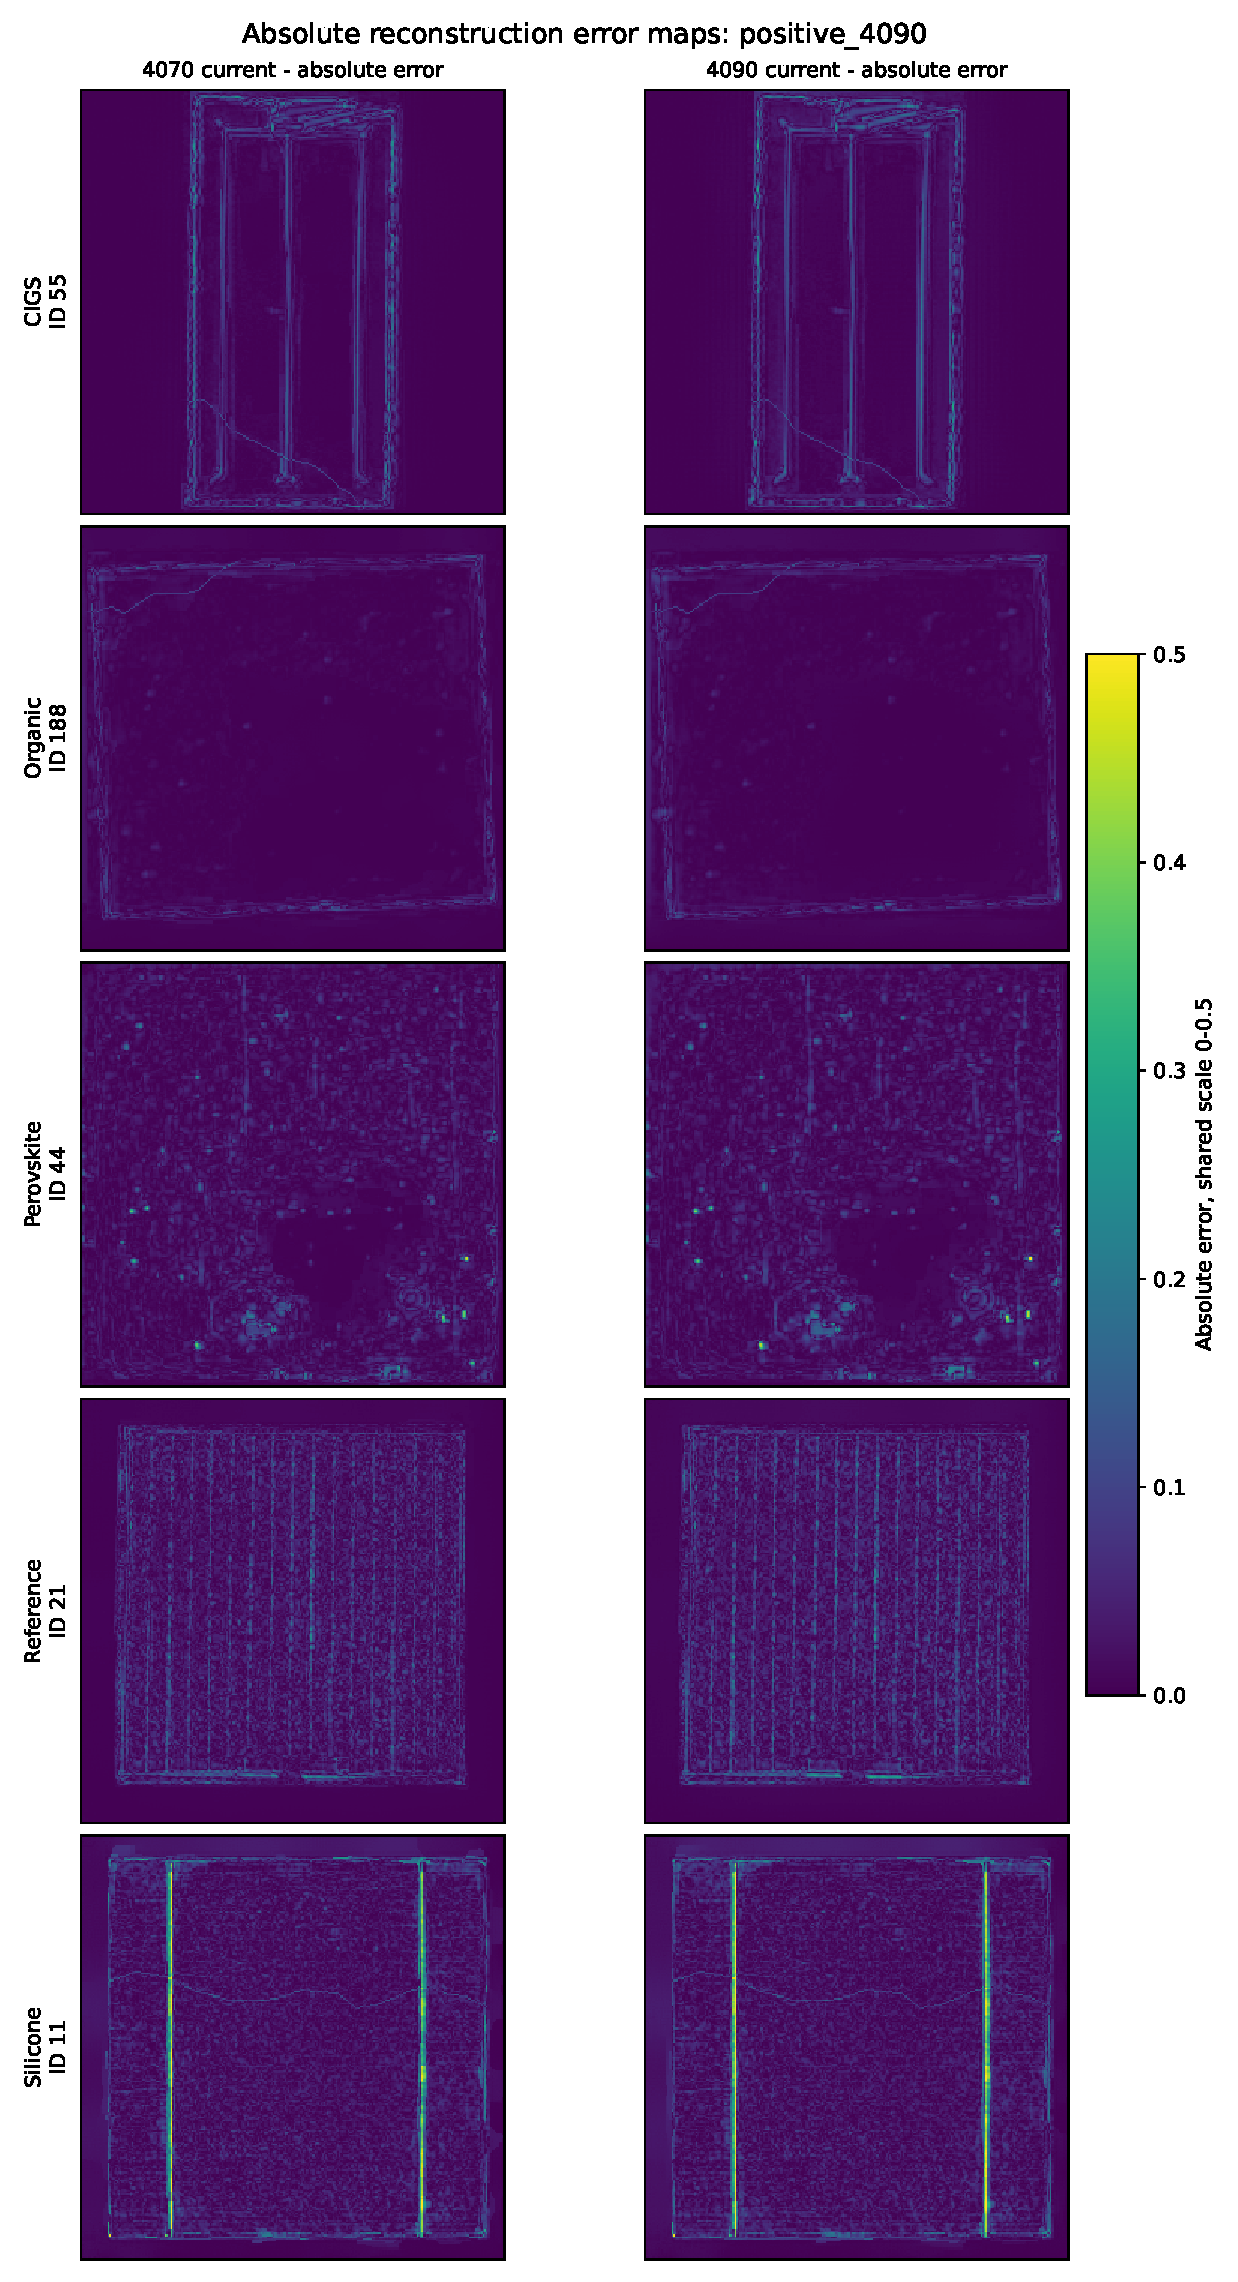
\includegraphics[width=.56\linewidth]{figures/absolute_error_positive_4090.pdf}
\caption{Absolute error positive 4090.}
\end{figure}\clearpage
\section{Performance impact and training safety}
The experiment used physical RTX 4070 (CUDA device 0), with approximately 10.6~GiB free VRAM before launch. Only the frozen current checkpoints were evaluated; old checkpoint results were reused. The 200 reconstructions (100 acquisitions times two current models) finished between 14:11:53 and 14:14:42 UTC without GPU OOM or errors, and all three ongoing training processes were observed alive afterwards. The evaluation paused 0.5 seconds per image and used a low CPU scheduling priority.

The 4070 training monitor recorded median 2.30 seconds/step during the 15 minutes just before evaluation, 2.33 during the three minute evaluation window and 2.30 in the three minutes after. This represents a short-term increase of approximately 1.3\% while evaluating, returning to baseline afterwards; it is not a complete controlled throughput experiment. The original 4090 and 3-by-56 training were not touched.
\section{Interpretation, limitations, and next steps}
\begin{enumerate}[leftmargin=*]
\item \textbf{Evidence of continued improvement.} The 4070 epoch-17 checkpoint delivers better reconstruction metrics than its epoch-7 checkpoint on exactly matched measurements. The paired change has a negative MSE interval that excludes zero and positive PSNR, SSIM and HaarPSI changes.
\item \textbf{4090 is not uniformly improving.} Its epoch-23 checkpoint slightly improves the mean MSE over epoch 22, but loses mean PSNR and SSIM. These discrepancies are compatible with image-dependent changes in loss distribution and merit investigation with fixed validation acquisitions and visual examples. They do not establish that the hardware itself is worse.
\item \textbf{Cross-model comparisons.} The current 4070 leads the sample averages, particularly PSNR and HaarPSI. However, some image categories and low sampling-ratio cases favor 4090 in MSE, and the overall head-to-head MSE interval contains zero. Avoid saying the 4070 is universally better.
\item \textbf{Selection and reuse limitations.} The 50 images were held out from model fitting, but all came from a test set already examined on 27 October. Repeated inspection may bias research decisions. The 4090 uses a differently distributed, stochastic validation procedure and an unequal number of training updates; neither model was trained under a controlled single-factor intervention. All images originate from the same synthetic PCM generator, not unseen physical acquisitions.
\item \textbf{Recommended next analysis.} Compare future checkpoints at predeclared epoch milestones on a \emph{fixed, separate validation acquisition set}; reserve untouched data for the final claim. To test causal hypotheses about optimizer versus noise schedule, run controlled retraining with common settings. Keep observing both running jobs without altering this experiment's frozen data.
\end{enumerate}
\appendix\section{Selected test image IDs and reproduction}
\begin{longtable}{lp{.74\linewidth}}\toprule Category & Fixed random sample IDs \\ \midrule\endhead
CIGS & 55, 79, 254, 279, 331, 376, 623, 710, 821, 933 \\
Organic & 188, 218, 232, 249, 364, 501, 727, 762, 807, 968 \\
Perovskite & 44, 55, 188, 254, 279, 333, 610, 611, 767, 786 \\
Reference & 21, 232, 294, 301, 331, 333, 370, 558, 608, 681 \\
Silicone & 11, 31, 79, 188, 307, 414, 527, 610, 793, 805 \\
\bottomrule\end{longtable}
The bundled \texttt{protocol\_manifest\_50.json} contains checkpoint epochs, steps, hashes and selection provenance. \texttt{evaluate\_current\_50.py} regenerates paired PCM acquisitions using the earlier test's seed namespace and checks pattern and measurement hashes. \texttt{summarize\_50.py} reconstructs the tables and paired bootstrap intervals. \texttt{make\_figures.py} generates both vector PDF and PNG charts. \texttt{all\_paired\_results\_old\_new.csv} contains all 100 acquisitions and all four checkpoint metric sets. The old full-test data have not been overwritten. The LaTeX source refers to the accompanying \texttt{figures/} PDF files and can be compiled with \texttt{latexmk -pdf}.
\section{Machine-readable source files}
\begin{itemize}[leftmargin=*]
\item \texttt{summary\_50.json}: overall results, per-category means, paired uncertainty, win counts, ratio stratification.
\item \texttt{all\_paired\_results\_old\_new.csv}: complete measured per-acquisition data for four frozen model checkpoints.
\item \texttt{protocol\_manifest\_50.json}: original and current checkpoint hashes, random sampling and test-reuse caveats.
\item \texttt{figures/}: nine PDF plots and matching PNG previews; the reconstruction/absolute-error panels use common display scales.
\item The five \texttt{current\_CATEGORY.csv} and ten \texttt{example\_CATEGORY\_REGIME.npz} files are also preserved in the run directory on tuni.
\end{itemize}
\end{document}
